%%%%%%%%%%%%%%%%%%%%%%%%%%%%%%%%%%%%%%%%%%%%%%%%%%%%%%%%%%%%%%%%%%%%%%%%
% Plantilla TFG/TFM
% Escuela Politécnica Superior de la Universidad de Alicante
% Realizado por: Jose Manuel Requena Plens
% Contacto: info@jmrplens.com / Telegram:@jmrplens
%%%%%%%%%%%%%%%%%%%%%%%%%%%%%%%%%%%%%%%%%%%%%%%%%%%%%%%%%%%%%%%%%%%%%%%%

\chapter{Marco Teórico}
\label{marcoteorico}

\section{Historia}
El mundo de los videojuegos va, en muchas ocasiones, de la mano con el \gls{ml}, debido a que es difícil desarrollar un algoritmo de \gls{ia} diseñado en los juegos en los que tienes que enfrentarte contra la máquina, y además, que este se ajuste a diferentes niveles de dificultad, para poder ajustarla según la habilidad del jugador. Sin entrar en profundidad de lo que hablaremos en los siguientes apartados, porque contaremos la historia de los motores, los videojuegos, y la \gls{ia}, he de mencionar algunos ejemplos de juegos emblemáticos que ilustren cómo ha sido la progresión a lo largo del tiempo. 
\begin{itemize}
	\item Tetris, es un juego del tipo puzle, que fue lanzado en 1984. Este juego no requiere de \gls{ia} ya que no tiene enemigos, la mecánica del juego reside en ser capaz de resolver el problema espacial y no existe un rival dentro del propio juego, solo has de tratar de no dejar huecos colocando piezas con distintas formas que aparecen en la parte más alta de la pantalla de con una de las formas aleatoria.\footnote{Para entender mejor el juego, puede ser visualizado en \url{https://www.youtube.com/watch?v=wnber_J6uSA}}
	\begin{figure}[h]
		\centering
		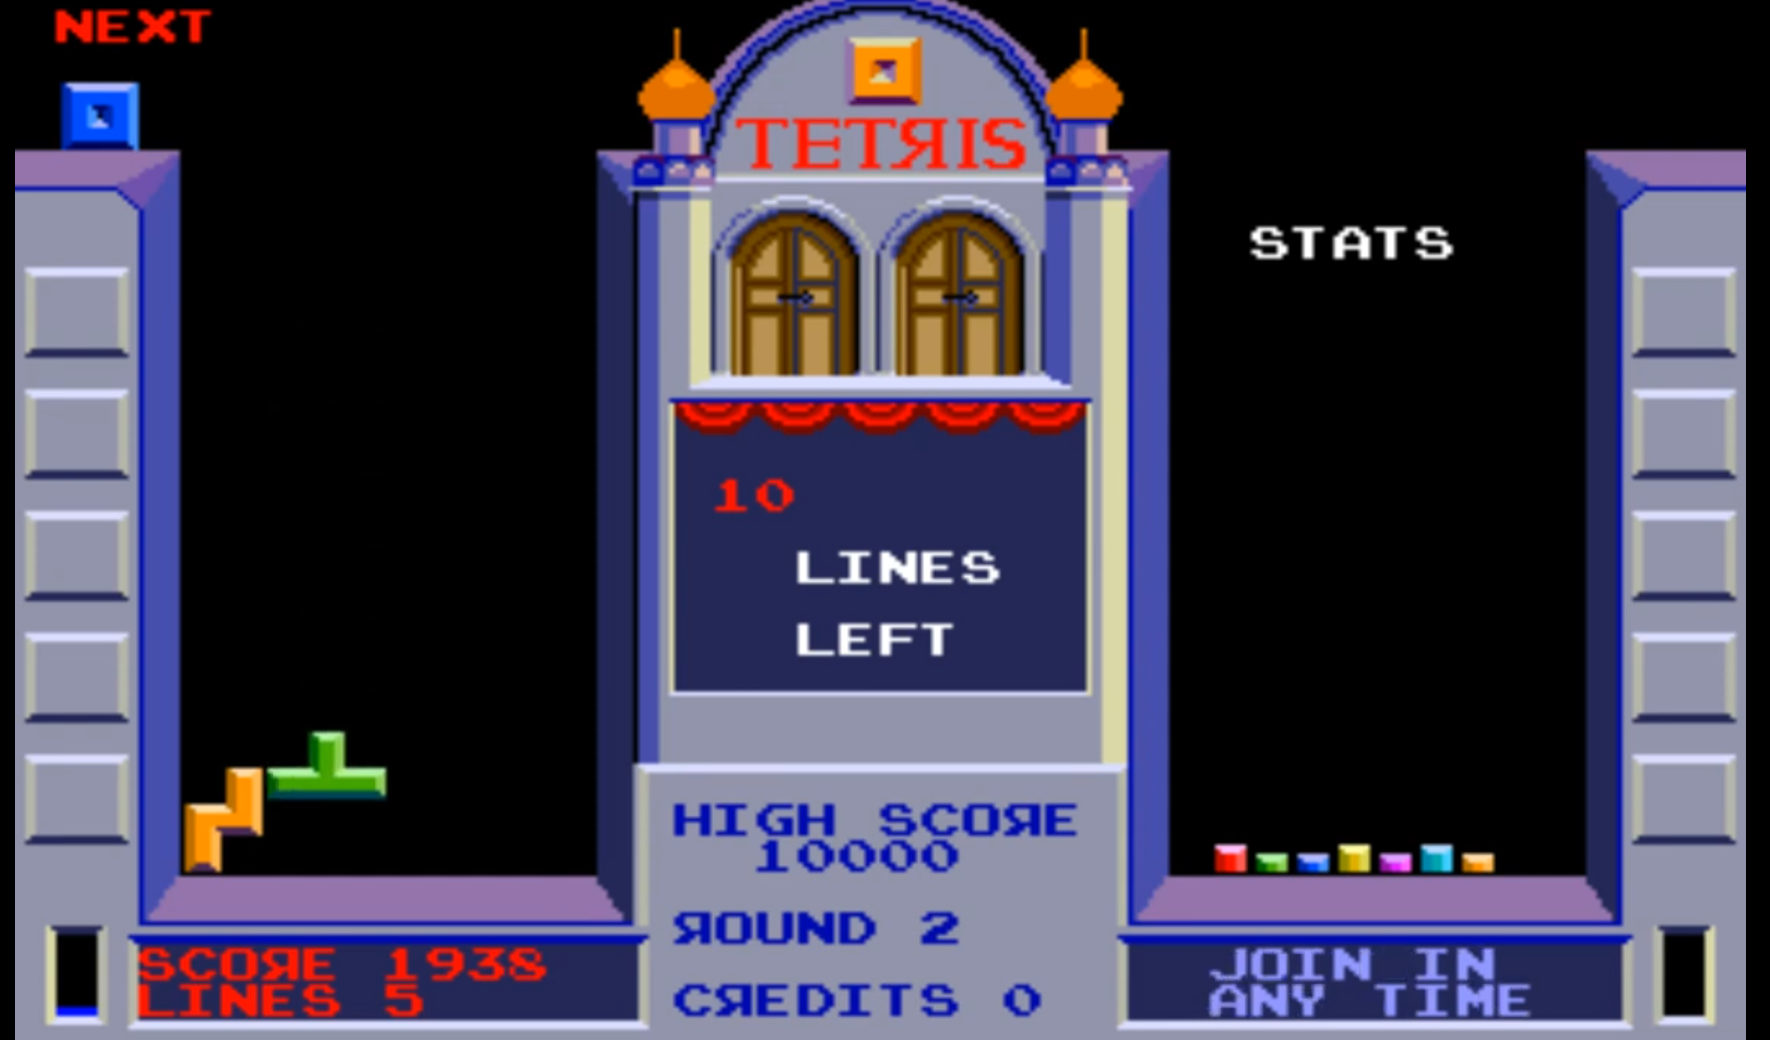
\includegraphics[width=15cm]{archivos/imagenes/tetris-1984.png}
		\caption{Tetris 1984.}
	\end{figure}
	\item Mario Bros, es un juego de tipo plataformas. Fue lanzado en 1983, en su primera versión, pero gracias al éxito que tuvo le siguió una larga saga de continuaciones del mismo y otras versiones con el mismo personaje principal y secundarios en las que el juego no trataba de lo mismo. En este juego sí que te encontrarás con personajes, has de enfrentarte a ellos, pero como el atractivo principal del juego es llegar a la meta moviéndote, la inteligencia de los mismos no requiere de ser muy compleja. Todos los personajes que aparecen tienen un comportamiento programado (también conocido como \gls{ia} diseñada), como moverse de lado a lado, salir de una tubería después de cierta cantidad de segundos, etc. Lo importante es que, aún con la presencia de enemigos, no era necesario una \gls{ia} muy desarrollada.\footnote{Para entender mejor el juego, puede ser visualizado en \url{https://www.youtube.com/watch?v=ly8DofqCuOs}}
	\begin{figure}[h]
		\centering
		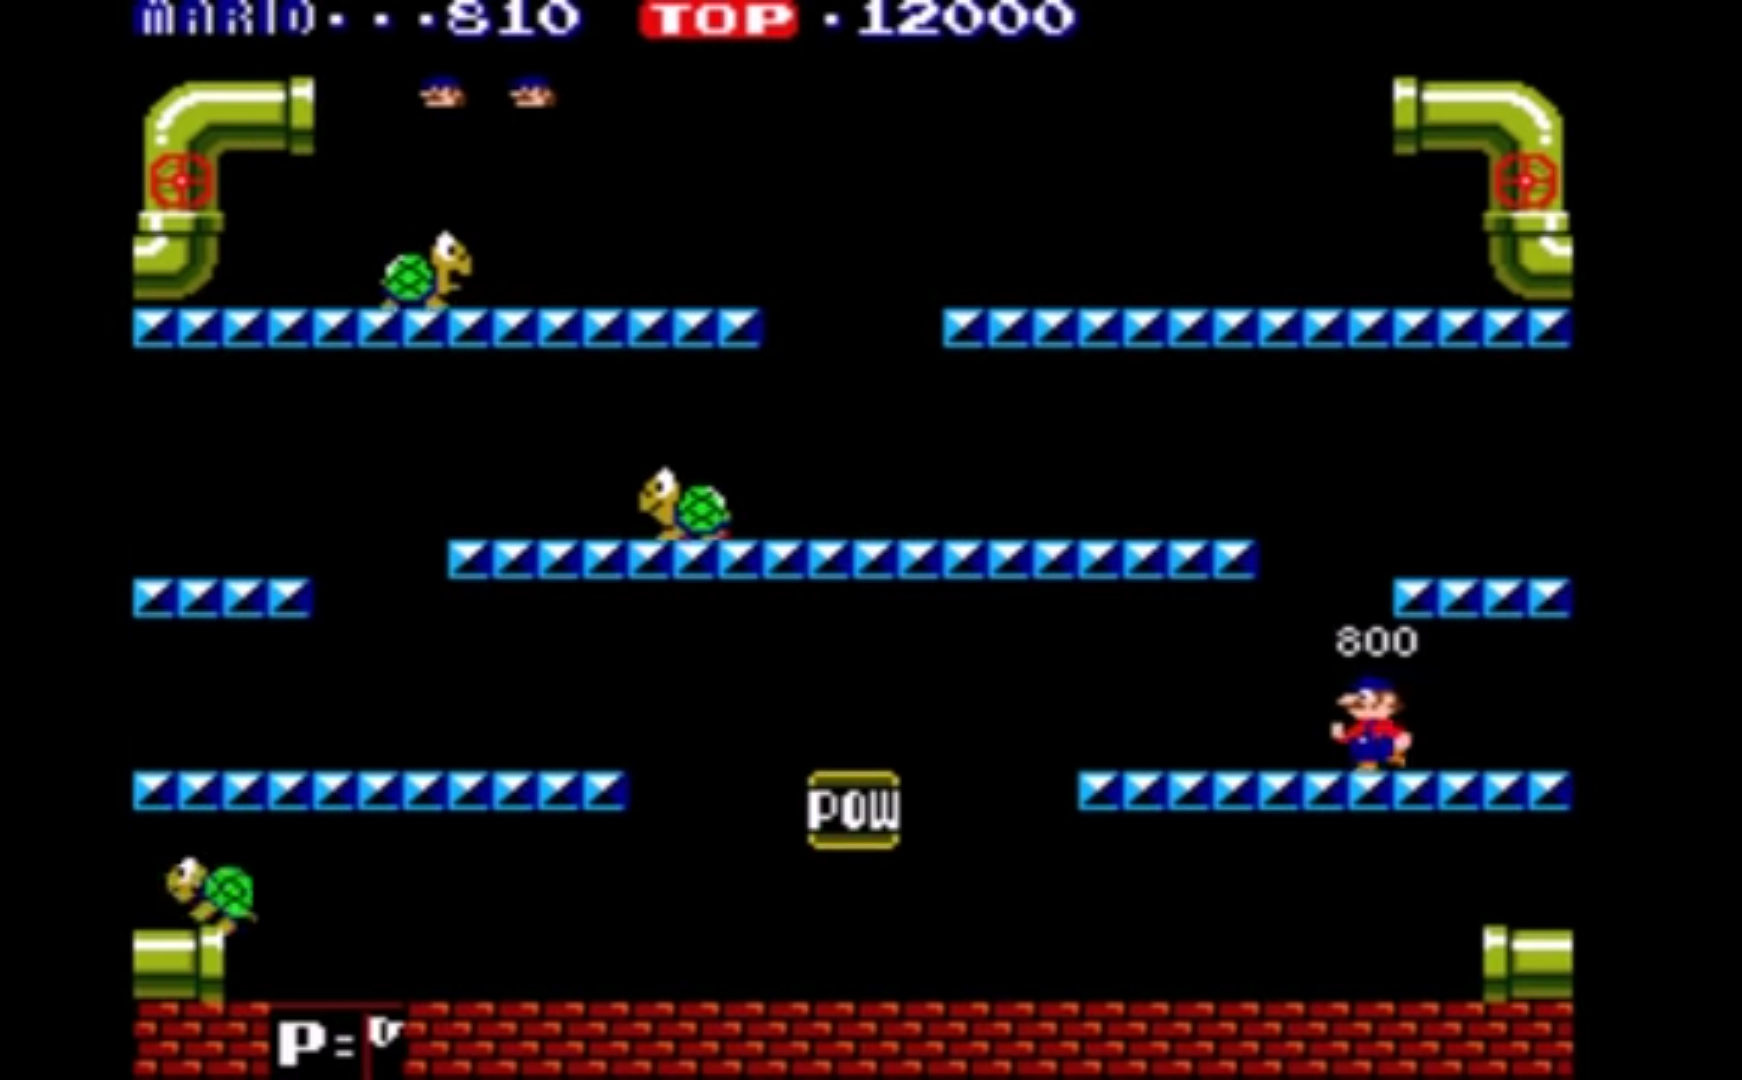
\includegraphics[width=15cm]{archivos/imagenes/mario-bros-1983.png}
		\caption{Mario Bros 1983.}
	\end{figure}
	\item Pokemon Red, Pokemon Green y Pokemon Blue. Los tres fueron lanzados en 1996, y son prácticamente iguales pero con sutiles diferencias. Estos juego son del tipo \gls{rpg}, es decir, que te introduce en la vida de un personaje, y has de jugar como si fueras tú el que toma y sufre las decisiones tomadas. A diferencia de Mario Bros, que tenías que moverte en una sola dirección y saltar, aquí te moverás en dos direcciones, y por lo tanto, los \gls{npc} también, pero estos siguen sin presentar ningún tipo de inteligencia avanzada, ya que normalmente siguen patrones en su camino que ya han sido programados, y los ataques que lanzan los Pokemon enemigos en los combates parecen ser aleatorios.\footnote{Para entender mejor el juego, puede ser visualizado en \url{https://www.youtube.com/watch?v=C034iux-EJ8}}
	\begin{figure}[h]
		\centering
		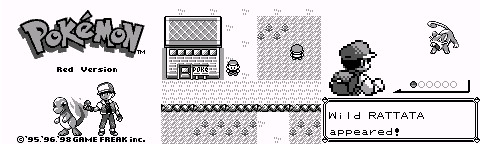
\includegraphics[width=15cm]{archivos/imagenes/pokemon-red.jpg}
		\caption[Pokemon Red.]{Pokemon Red\footnotemark.}
	\end{figure}
	\footnotetext{Imagen en la web retrospilling.no \url{https://retrospilling.no/2015/02/litt-om-pokemon/}}
	\item Left 4 Dead es un juego de supervivencia, y fue lanzado en 2008. Se trata de un juego de zombies en el cual vas con un equipo de cuatro personas, es aquí donde entra la \gls{ia}. Puedes jugar con tres amigos más, pero el juego también está hecho para jugar solo, por lo que los otros personajes requieren una inteligencia para ayudarte a completar los desafíos. No se conoce a ciencia cierta cómo está programado, pero se puede deducir que los \gls{npc} no tienen inteligencia para la búsqueda de rutas(pathfinding es el término más conocido) porque las rutas ya están definidas en el juego, pero sí cuando disparar, salvarte, etc.  mientras que los enemigos parecen comportarse siempre de la misma manera. Por lo que Left 4 Dead es el primer juego que tiene una \gls{ia} compleja de entre los que he mencionado hasta ahora.\footnote{Para entender mejor el juego, puede ser visualizado en \url{https://www.youtube.com/watch?v=oIHNW-cSGHI}}
	\begin{figure}[h]
		\centering
		
\includegraphics[width=15cm]{archivos/imagenes/Left-4-Dead.jpg}
		\caption{Left 4 Dead, primera versión.}
	\end{figure}
	\item League of Legends es un juego más actual, jugable en PC y fue lanzado en 2009. Pero además, ha sido lanzada una versión independiente para móviles en el año 2020. Este juego se trata de un \gls{moba}, en el cual te enfrentas con tus compañeros, contra otros cuatro oponentes y has de derrotar la torre principal del enemigo para ganar, teniendo como obstáculos no solo a los oponentes, sino también a minions y las propias torres que se encargan de dispararte. Podría parecer que no hay ninguna \gls{ia}, pero lo cierto es que sí que se aplica un campo que es el de la búsqueda de la ruta más rápida. Esto está presente en muchos otros juegos, y es cierto que es un campo de la \gls{ia}, pero no requiere de aprendizaje, por lo que no ha de ser entrenado con técnicas de \gls{ml} y no es necesario programar redes neuronales para el uso de la misma. Esto es usado tanto por los minions, para moverse por el mapa, como por el jugador, que se mueve haciendo clicks donde quiere ir, y no con AWSD como es típico en los videojuegos más actuales.\footnote{Para entender mejor el juego, puede ser visualizado en \url{https://www.youtube.com/watch?v=PZ2ORXhIrVU}}
	\begin{figure}[h]
		\centering
		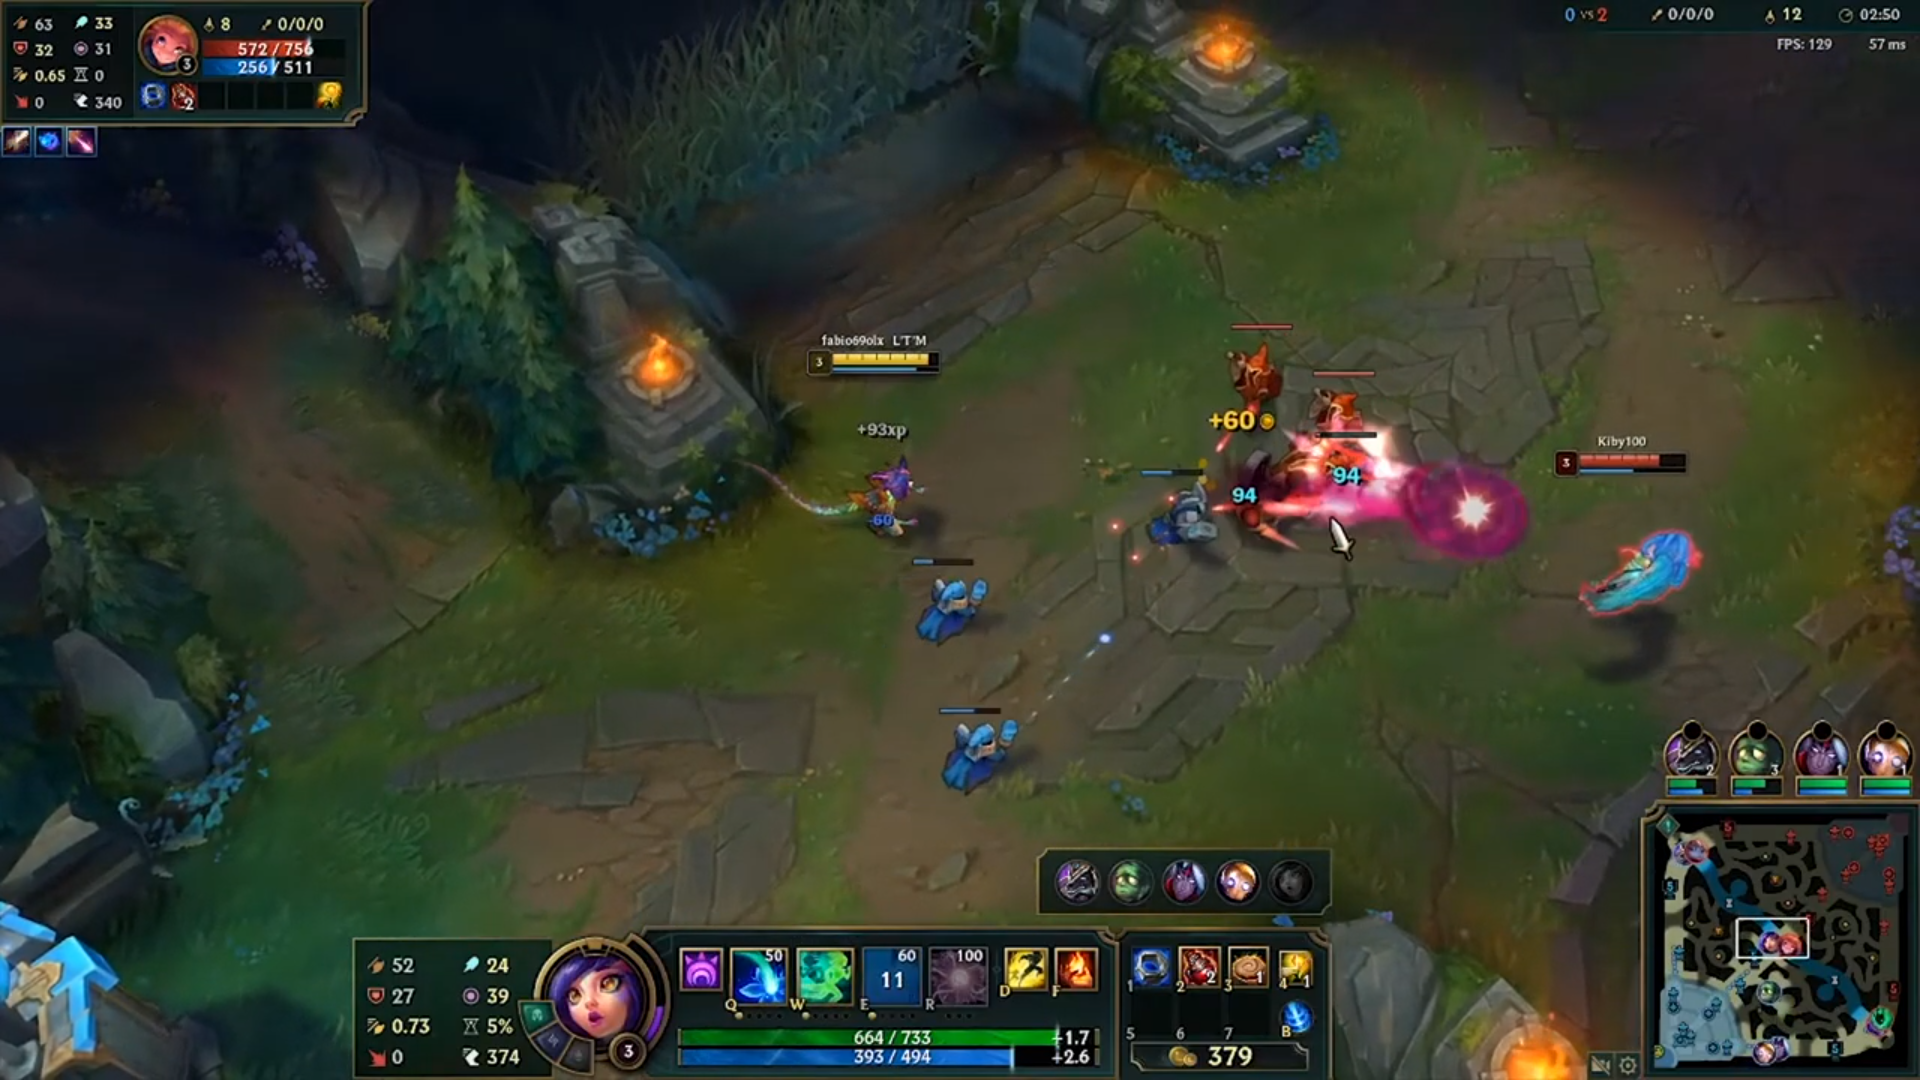
\includegraphics[width=15cm]{archivos/imagenes/league-of-legends.png}
		\caption{League of Legends.}
	\end{figure}
\end{itemize}

De todos los juegos mencionados anteriormente, no se puede saber si fueron creados utilizando un motor de videojuegos, salvo si los autores de los mismos desvelasen los detalles, pero es fácil de deducir que los más antiguos no utilizaron un motor, sino que fueron creados desde cero, pero los que tuvieron sagas reutilizarían parte del código, con lo que muchas de las partes del código las acabarían integrando en un motor, para la posterior creación de los siguientes juegos de la saga. Mientras que todos los juegos actuales utilizan un motor, debido a que ya existen motores muy buenos, y gastar el recursos del desarrollo en algo que ya existe haría perder beneficios a la empresa desarrolladora del videojuego.

\section{Motor de videojuegos}
El motor de videojuegos es el software encargado de que el desarrollador de videojuegos pueda programar estos sin tener que preocuparse por lo cómo se gestionan las entidades del juego, solo pensando en la lógica de las mecánicas, y demás aspectos del videojuego. 
\\
Después de la creación de los primeros juegos, los programadores de videojuegos se dieron cuenta de que había partes del desarrollo que se repetían. Algunas como la creación y destrucción de entidades entre otras cosas. Por eso, las empresas dedicadas a ello, comenzaron a diferenciar la parte de la creación del juego con la del motor, ya que, con un mismo motor, se podrían hacer distintos videojuegos.
\\
Pero fue en los años 90, con la creación de videojuegos en 3D donde se acuñó el termino de ``motor gráfico''. Fue debido a que en la mayoría de los casos, el motor no solo se encargaba de la gestión de entidades sino también de la renderización del juego, así que de esta forma se entendía mejor para qué servía esta pieza de software. El que se conoce como primer motor gráfico para PC fue Freescape Engine, que se utilizaba para hacer juegos de disparos en primera persona, esto es debido a que los primeros juegos en popularizarse para PC fueron de este género.
\\
Realmente los motores gráficos no solo sirven para crear juegos, así que con el tiempo, estos motores se empezaron a utilizar no solo para videojuegos, sino también para desarrollar aplicaciones que tengan que ver con simulación de la vida real, como pueden ser aplicaciones arquitectónicas, educación, simuladores para aprender a conducir, y un largo etcétera.

Actualmente, en el mundo hay muchos motores de videojuegos, algunos públicos de pago (Unreal Engine, Unity, etc.), utilizado sobretodo por desarrolladores indie, otros privados para que una empresa lo utilice o reutilice para hacer sus videojuegos, e incluso cabe mencionar Godot Engine por ser el más famoso entre los motores de libre uso, sin coste para el desarrollador. En general, el mundo de los motores es un mundo bastante maduro, aunque de vez en cuando surjan mejoras.
\\
Y con tanta oferta de motores, es obvio que estos existen porque el mundo de los videojuegos se ha ampliado, hasta tal punto que existen de todo tipo y para una gran cantidad de plataformas. En ordenadores existen plataformas de venta de videojuegos como Steam o Epic Games entre otros, donde puedes encontrar infinidad de títulos, entre los que me gustaría destacar Minecraft, Hollow Knight y Braid, demostrando que en el mundo de los videojuegos no hace falta ser enormes multinacionales para hacer juegos tremendamente entretenidos y con mecánicas originales. Mientras que en plataforma móvil, la mayoría de juegos los adquirirás en el  \textit{marketplace}\footnote{Un \textit{marketplace} es una aplicación del sistema operativo desde la cual puedes encontrar y descargar otras tantas aplicaciones.} del sistema operativo que use tu móvil, y por lo general, el mercado está copado de juegos casual con los que pasar un rato, pero también hay algunas joyitas, ya que las empresas de videojuegos se han dado cuenta de que es un mercado en crecimiento, Monument Valley, Pixel Dungeon o juegos ya famosos en PC que han portado su juego a versión móvil como League of Legends, Call of Duty o Mario Kart.

En este \gls{tfg} voy a usar uno de creación propia, en base a las lecciones aprendidas en el curso de \citep{CursoMotorC++}, pero el mercado de motores de videojuegos es tan extenso que hay muchos que podrían ser usados para el proyecto. Pero como la motivación del mismo es desarrollar las tecnologías de un videojuego desde cero, me he decidido por desarrollar el mío en el lenguaje C/C++ con el uso de algunas pocas librerías externas.

\section{Videojuegos}
Fueron creados como entretenimiento, mediante el uso de un hardware que actúa como entrada en el juego los interpreta y el juego actúa según la lógica programada. Los primeros datan de los año 1952 y 1958 (Tres en raya y Tennis for Two respectivamente). Pero con el paso de los años han progresado, llegando a ser más complejos. 
\\
Con el auge de las consolas, muchas empresas surgieron y crearon videojuegos, como Nintendo con su mundialmente conocido Mario Bros, Game Freak con Pokemon, y un largo etcétera. 
\\
Después de varios años, y la creación de motores de videojuegos, la gente empezó a poder tener ordenadores en casa. Surgen distintas tecnologías como Flash Player para navegadores, con lo que alguien con conocimientos de programación podía crear su videojuego sin preocuparse del renderizado, y compartirlo con el resto de usuarios de ordenador que tuvieran esta tecnología instalada en su navegador.

Conforme fue haciéndose más grande la industria de los videojuegos, algunas empresas empezaron a comercializar su motor de videojuegos, no solo vendiéndolo a otras grandes empresas que pudieran comprarlos, sino a pequeños desarrolladores, llamados desarrolladores indie\footnote{El término proviene de desarrollador independiente, que no trabaja para una empresa sino que crea sus propios juegos.}, los cuales no pueden permitirse costes tan altos. Pero si una empresa que desarrolla el motor consigue vender licencias más baratas a una cantidad muy grande de gente, hace que también sea rentable el desarrollo de motores de videojuegos. A causa de esto, y cuando Steam permitió vender juegos a los desarrolladores indie en su plataforma, aumentó la cantidad de videojuegos en el mercado.

Otra industria que ha crecido en los últimos años de manera exponencial son los videojuegos para móvil. A pesar de que con los primeros móviles ya se podía jugar a juegos más sencillos que ya venían preinstalados, como el Snake, el verdadero auge ha sido con la popularización de los sistemas operativos Android e iOS. Estos dos sistemas operativos son los que dominan en la actualidad todo el mercado de los móviles, y vienen con un marketplace instalado, cada uno el suyo. Tanto la Play Store (de Android) como la App Store (de iOS) permiten a cualquier desarrollador subir sus propios videojuegos\footnote{Para subir cualquier aplicación a una de ellas has de cumplir unos requisitos. Ya que es un servicio centralizado, tiene que pasar unos estándares de seguridad para no ser utilizado como puerta de entrada de virus o programas no deseados.}, con lo que se expandió aún más el mercado de los videojuegos. De hecho, el mundo de los videojuegos móviles es tan popular que algunos motores de videojuegos te permiten compilar tu juego tanto para móviles como para ordenador, pudiendo de esta manera, rentabilizar aún más tu juego al abrirte a un mercado mayor, y esto ha hecho que aún más gente se anime a dedicarse a ser desarrollador.

Aunque actualmente, en el año 2021, la mayoría de juegos son construidos tanto para consola como para ordenador, por lo que con un ordenador puedes jugar casi todos, al principio se diseñaban máquinas especialmente para jugar, véase Atari 2600, NES, Game Boy, Mega Drive, Nintendo 64. Es decir, los juegos se hacían especializados para el hardware de la máquina, sin embargo, la popularización de los ordenadores domésticos hizo que cada vez haya que hacer los juegos más genéricos, y si una máquina en concreto necesita de una tecnología distinta, el motor se encarga de usarla a la hora de la compilación.

\section{\glsentrylong{ia}}
Cuando hablamos de \gls{ia} nos referimos a máquinas imitando comportamientos inteligentes. Esta definición es dada en 1955 con el nacimiento de la \gls{ia}. Pero si hablamos de \gls{ia} podemos estar hablando de distintos campos, ya que es un término muy genérico. Más concretamente, en este \gls{tfg} tratamos el campo del \gls{ml}.
\\
Para comprender la diferencia entre un comportamiento programado y un comportamiento aprendido me gustaría citar a Stuart J. Russell y Peter Norvig, \textit{"un agente aprende cuando su desempeño mejora con la experiencia; es decir, cuando la habilidad no estaba presente en su genotipo o rasgos de nacimiento"}.\footnote{Cita escrita en el libro \textit{Inteligencia Artificial: Un Enfoque Moderno} de los autores anteriormente mencionados.} Por lo tanto, podremos diferenciar dentro del mundo de la \gls{ia} (que es una lógica aplicada por una máquina), al \gls{ml} (que es un comportamiento, que además de ser aplicado por una máquina, ha de ser aprendido). Se hablará más en detalle sobre el \gls{ml} en el apartado \ref{importancia ml}.

La primera tecnología que permitía a una máquina tener \gls{ia} que aprendiese fue el perceptrón, presentado en 1959 por Rosenblatt. El perceptrón resuelve muy bien problemas generales, y de forma perfecta problemas que sean linealmente separables, como puede ser una puerta OR o una puerta AND, pero pronto se dieron cuenta de sus limitaciones, dado que una puerta lógica XOR no es linealmente separable, el perceptrón no funcionaba de forma correcta en estos casos. Este problema se solucionaría usando un segundo perceptrón, por lo tanto la lógica del programa depende de dos salidas, y sí que se podría separar.
\begin{figure}[h]
	\centering
	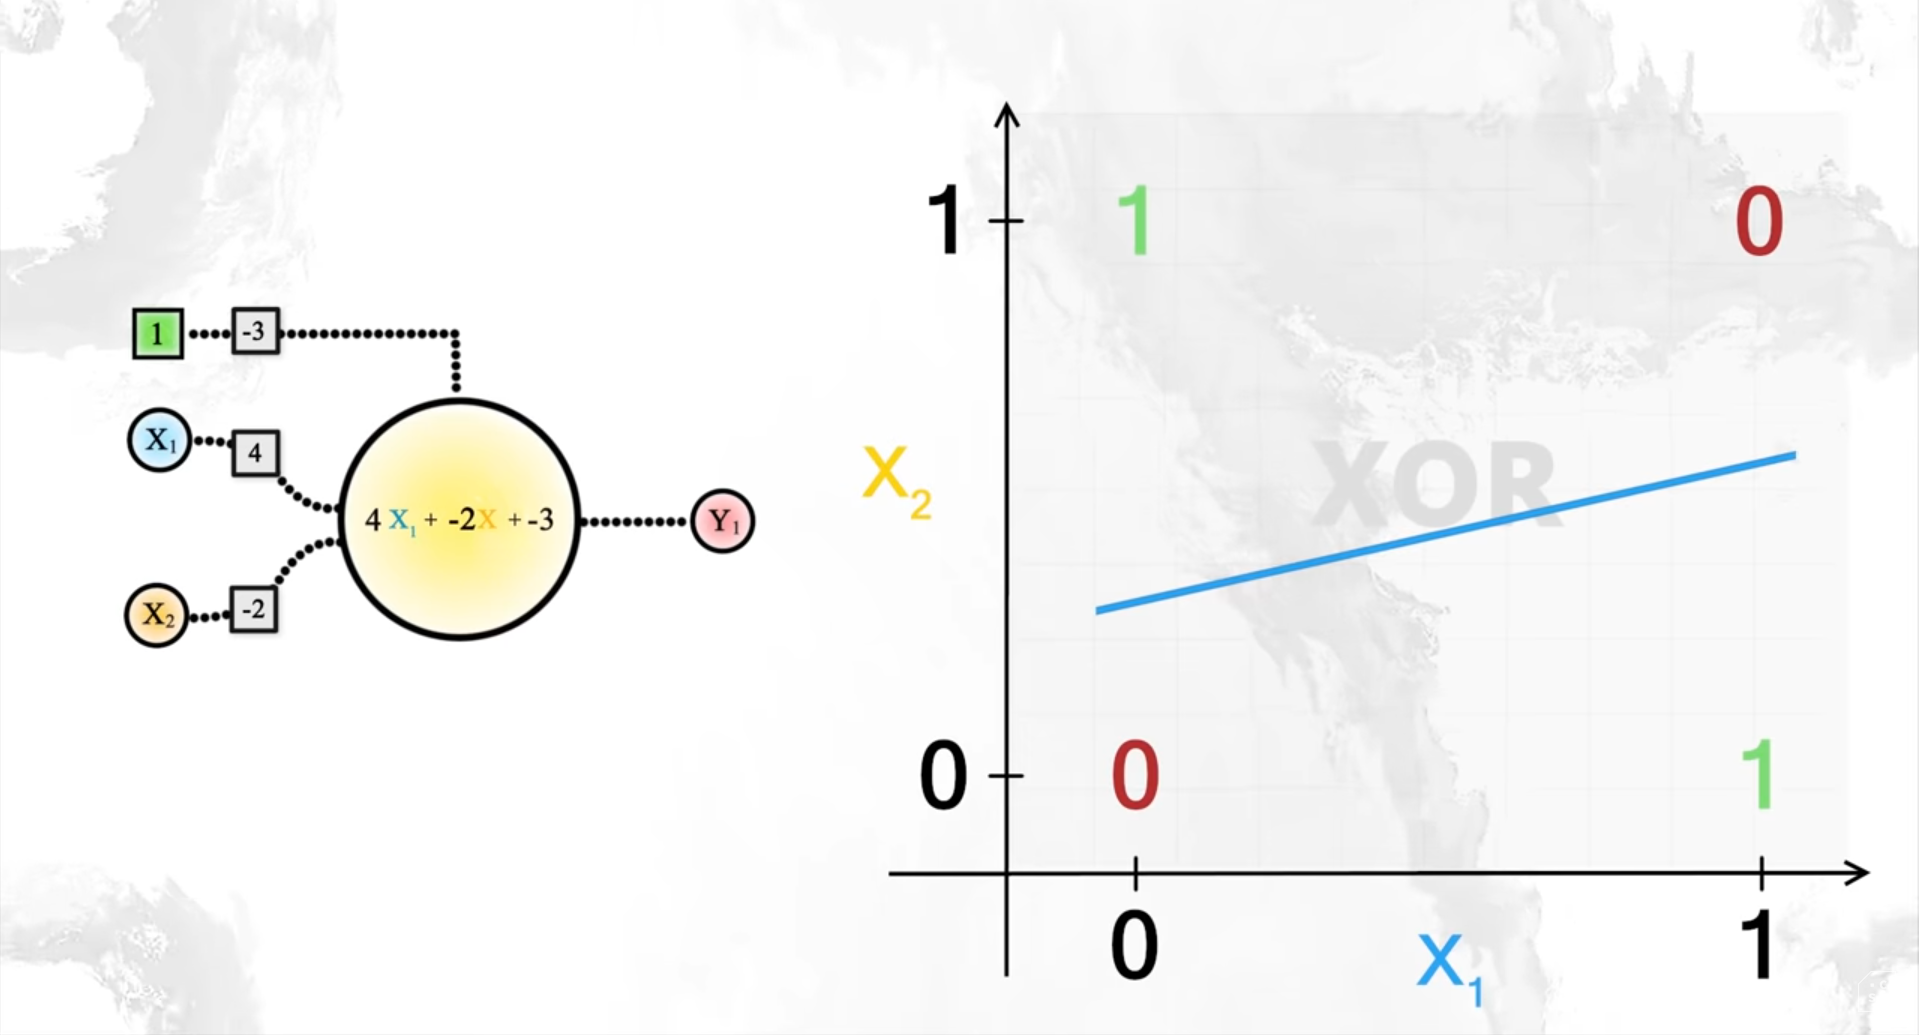
\includegraphics[width=15cm]{archivos/imagenes/problema-xor.png}
	\caption[XOR irresoluble por un solo perceptrón.]{XOR irresoluble por un solo perceptrón\footnotemark.}
	\label{XOR con un perceptron}
\end{figure}
\footnotetext{Desde el canal de YouTube de Carlos Santana \url{https://www.youtube.com/watch?v=MRIv2IwFTPg}}

Pero el perceptrón no es el único modelo dentro del mundo de la \gls{ia}, en 1940 Warren McCulloch y Walter Pitts crearon un modelo informático que se llamaba lógica umbral, esto es lo primero que se conoce sobre redes neuronales. Si bien, su lógica es parecida a la del perceptrón, tiene algunas diferencias. 

Dada la lógica del perceptrón, y resuelta la problemática de los problemas no separables linealmente, se crearon las redes de perceptrones, también llamadas \gls{mlp}. Con ellas se podían resolver problemas como el de la puerta XOR, pero pronto se dieron cuenta de sus limitaciones, y es que al final, el hecho de aplicar múltiples funciones aritméticas f(x) con sumas y multiplicaciones en cadena era equivalente a hacer una sola función aritmética f(x). Pero esto fue solucionado fácilmente cambiando la función de activación. Mientras que la función de activación de un perceptrón era una función escalonada, la función de activación de una neurona puede ser cualquier función matemática, las más comunes son la sigmoide, la ReLU, y la tangente hiperbólica. Esto es la principal diferencia entre un perceptrón y una neurona.
\\
Las limitaciones de las redes neuronales salieron a la luz después de hacer experimentos, ya que era demasiado costoso computacionalmente saber qué neurona dentro de la red neuronal había cometido el error, puesto que el método de búsqueda era por fuerza bruta, y esto supuso un gran parón en el mundo de la \gls{ia}, porque ajustar los pesos de la red manualmente era inviable para redes muy grandes y además porque el poder computacional en aquellos tiempos era más limitado.
\\
Pero en 1986 se inventó un algoritmo que era capaz de, en función de un error dado en la salida de la red neuronal, propagar el error hacia las neuronas de capas anteriores, de forma que cada una corregía su peso en la red neuronal en función de lo culpable que era en ese error. Su nombre es retropropagación, o como se le conoce por su nombre en inglés \textit{backpropagation}. 

Actualmente el mundo de las \gls{ia}, aunque existen sistemas muy complejos y completamente desarrollados, es un mundo en el que constantemente recibimos nuevas noticias de un sistema que mejora al anterior, o que consigue hacer cosas nunca antes vistas. Así que podríamos decir que es menos maduro y tiene muchísimo margen de mejora aún.
\\
Algunos de los frameworks más usados para desarrollar \gls{ia} actualmente son TensorFlow y Keras entre otros, debido a su potencial y su sencillo uso, ya que no tienes que ser un experto para poder usarlas y poder programar tú mismo la \gls{ia}.

\subsection{¿Cómo resolver el problema del perceptrón?}
Sabiendo que el problema del perceptrón, que sólo podía resolver problemas linealmente separables, y que juntando varios obtenemos lo que en inglés se llama \gls{mlp} y por lo tanto, podemos resolver problemas como la XOR, pero sigue existiendo limitaciones. ¿Cuáles son estas limitaciones y por qué se dan?
\\
Para resolver estas preguntas has de entender qué es lo que hace un perceptrón gráficamente, y no de forma analítica. Como vemos en la figura \ref{XOR con un perceptron}, tenemos un perceptrón de dos entradas y una salida, pero no solo eso, sino que esto significa que el total de pesos que contiene es dos, o lo que es lo mismo, el número de parámetros libres del modelo es dos. Por lo tanto, el perceptrón es representable en una gráfica bidimensional, como lo que se conoce por una recta. Si despejamos cualquiera de las dos variables, obtendremos la ecuación de la recta:
\begin{equation}
	y = m*x + n
\end{equation}
El siguiente paso es colocar las entradas del dataset en la gráfica. Como ya habremos despejado uno de los términos, ese será el que haga de ``y'', y el otro de ``x''. Como vemos de nuevo en la figura \ref{XOR con un perceptron}, el perceptrón $4*X_1 + -2*X_2 + -3$ representado por la recta en azul, no es capaz de separar los 1s y los 0s. Mientras que en la siguiente gráfica que es la que representa los valores de una puerta AND vemos que un solo perceptrón sí que es capaz de resolver el problema.
\begin{figure}[h]
	\centering
	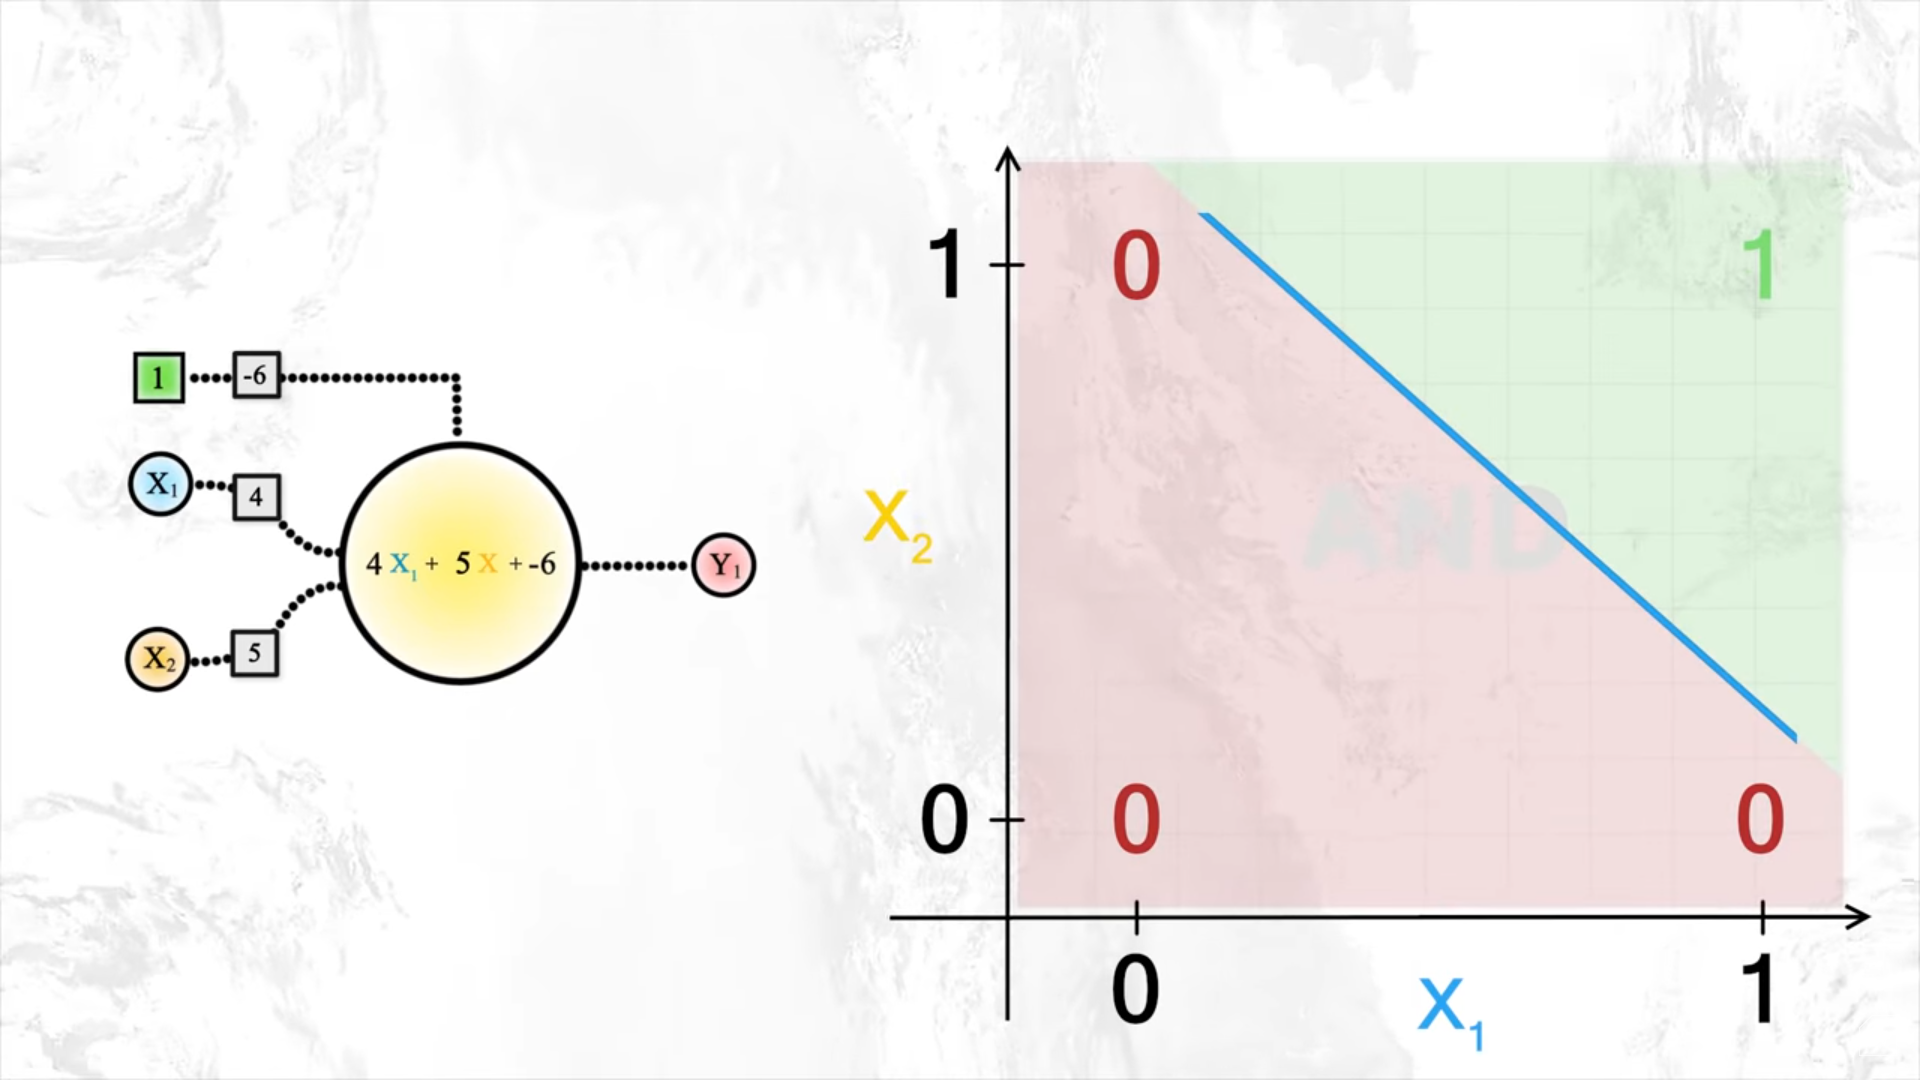
\includegraphics[width=15cm]{archivos/imagenes/perceptron-con-and.png}
	\caption[AND resuelta por un solo perceptrón.]{AND resuelta por un solo perceptrón\footnotemark.}
\end{figure}
\footnotetext{Desde el canal de YouTube de Carlos Santana \url{https://www.youtube.com/watch?v=MRIv2IwFTPg}}

Después de entender qué es un perceptrón gráficamente, una recta, es sencillo darse cuenta de que uno sólo no sería capaz de resolver el problema de la XOR, pero dos rectas sí que serían capaces de hacerlo, por eso es por lo que cobra sentido el \gls{mlp}. Pero este último también tiene sus limitaciones, que veremos en el apartado \ref{Redes Neuronales}.

\begin{figure}[h]
	\centering
	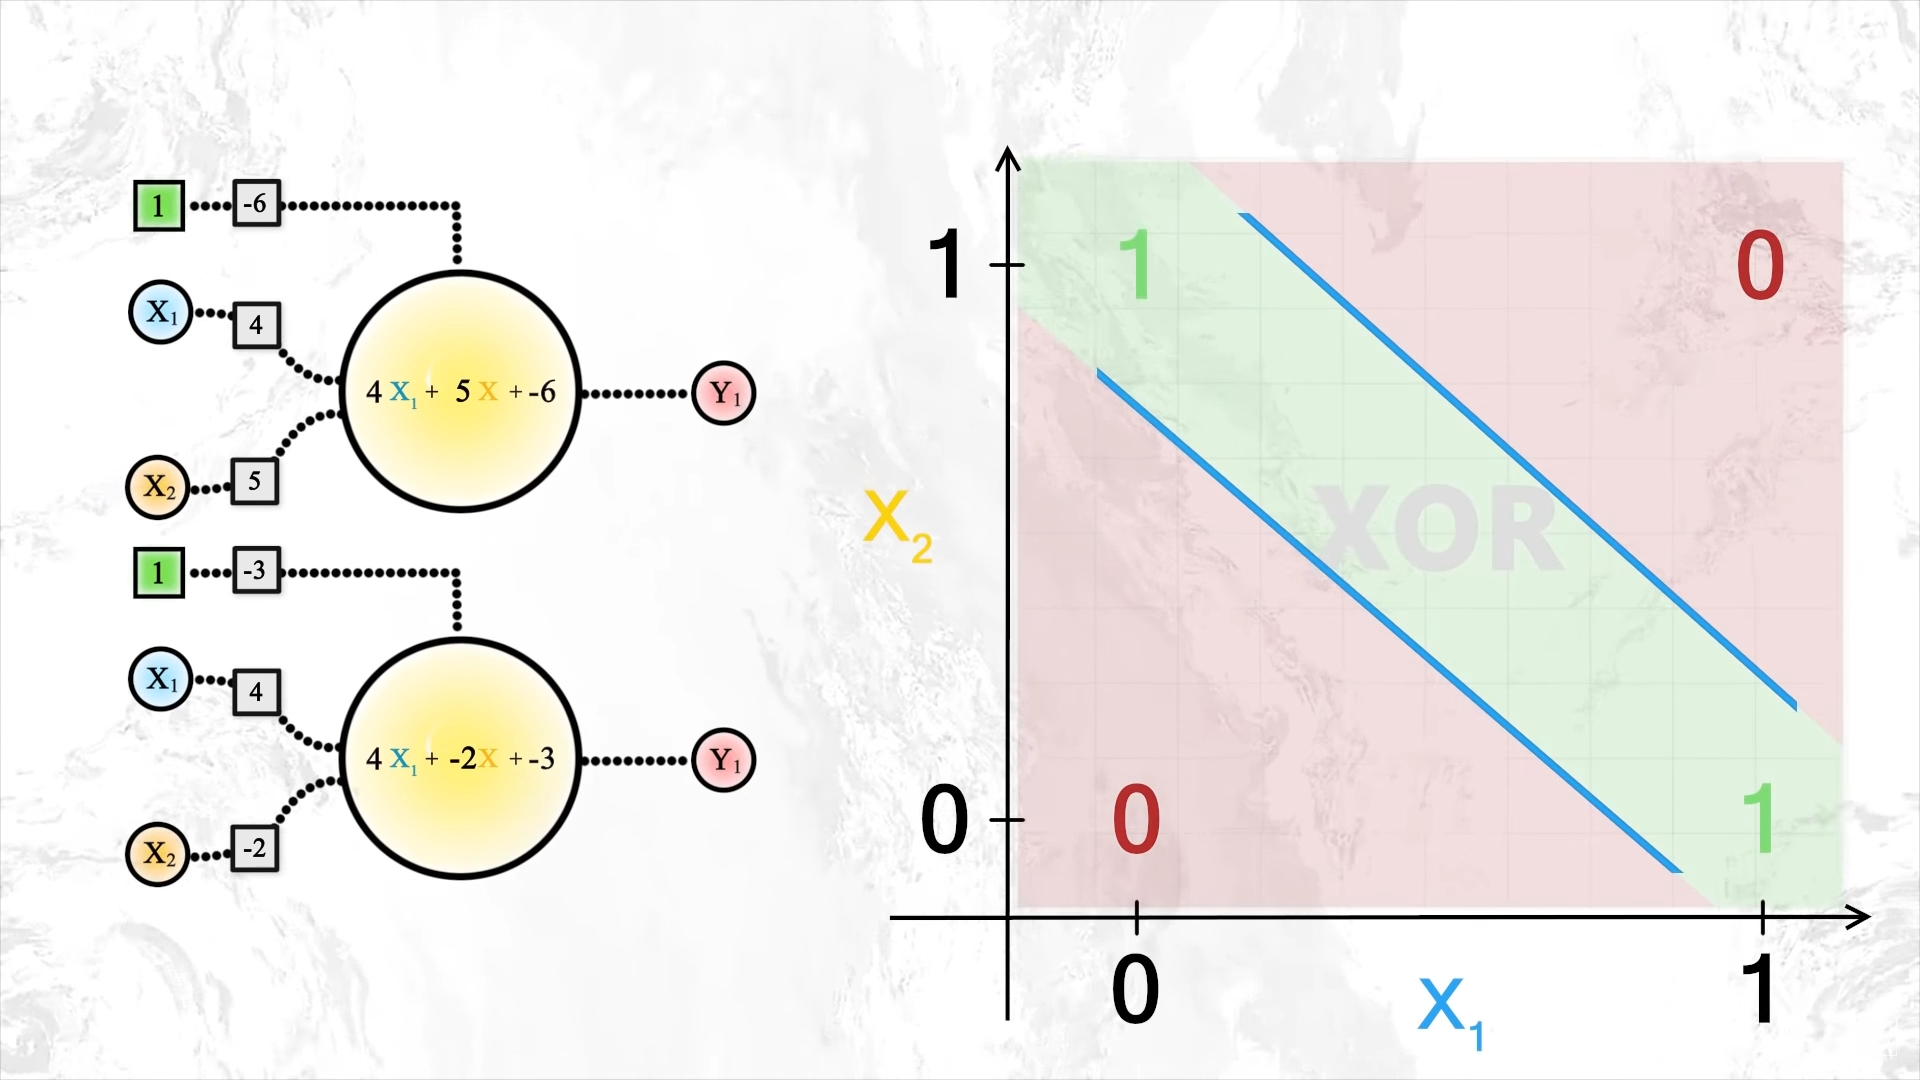
\includegraphics[width=15cm]{archivos/imagenes/problema-xor-resuelto.png}
	\caption[XOR resuelta por dos perceptrones.]{XOR resuelta por dos perceptrones\footnotemark.}
\end{figure}
\footnotetext{Desde el canal de YouTube de Carlos Santana \url{https://www.youtube.com/watch?v=MRIv2IwFTPg}}

\subsection{Importancia del \glsentrylong{ml}}
\label{importancia ml}
El \gls{ml} es un área tremendamente importante en la actualidad. No solo en el campo de los videojuegos como se desarrollará en este caso. También se aplica en distintos campos: tanto en motores de búsqueda, análisis de mercados, detección de enfermedades y muchos más. 
\\
Esto es debido a que estos problemas tienen complejidades suelen ser inasumibles con los algoritmos conocidos, porque se trata de complejidades NP-Hard, es decir, como mínimo, tan complejos como \gls{np}\footnote{Es el conjunto de problemas que pueden ser resueltos en tiempo polinómico por una máquina de Turing no determinista.}. 
\\
El \gls{ml} se encarga de resolver estos problemas, de tal manera que a partir de una pequeña parte de todo el espectro de datos que concierne al problema original \gls{np}, se consigue generalizar una o varias funciones que separan los datos de todo el espectro con el menor error posible.

Por muy avanzada que sea la \gls{ia}, todavía es necesario que la inteligencia de un humano intervenga para desarrollar un nuevo sistema enfocado en un aspecto en concreto. Esto es porque no existe una \gls{ia} capaz de programar un programa complejo, aunque sí se ha demostrado ya que existen \gls{ia} capaces de programar, como es el caso de GPT-3, que usa deep learning, un campo derivado del \gls{ml}.

De manera general, podemos decir que el verdadero potencial del \gls{ml} es la capacidad de analizar datos a la velocidad de un ordenador, y aplicar una lógica aprendida con esos datos para realizar predicciones.
\\
Sin embargo, es una tecnología con la que hay que tener mucho cuidado, debido a que se suele utilizar junto al Big Data, que es la forma en la que llamamos a recoger una gran cantidad de datos para analizarlos, ya que como estos datos no están revisados, estas máquinas inteligentes pueden verse afectadas por sesgos negativos. Como casos importantes tenemos el algoritmo de detección de fotos de Google, que identificaba a algunas personas negras como gorilas, o el bot de Twitter de Microsoft, que aprendió comportamientos racistas y machistas en base a estudiar el comportamiento de esta red. 

\subsection{Tipos de \glsentrylong{ml} }
La \gls{ia} es el nombre que se utiliza para englobar todos los campos donde una máquina se comporta de manera inteligente, por lo tanto, hay que concretar más. El tema que se trata en este \gls{tfg} es el \gls{ml}, que busca dotar a las máquinas de la capacidad de aprendizaje, mediante el análisis de datos empíricos de una situación en la que se pretende predecir el resultado de un dato que no está presente dentro de esa muestra, y por supuesto, predecir al mismo tiempo los que sí lo están. 
\\
La parte común que converge en todos los tipos de aprendizaje es la siguiente: la máquina genera una función aleatoria, y esta función produce una salida en base a los datos de entrada que le han sido suministrados. Esta salida será, en la mayoría de los casos, errónea (dado que la función se ha generado de manera totalmente aleatoria), y no se parecerá en nada a lo que queremos que aprenda, así que según la forma de analizar y corregir este error de salida, se distinguen varios tipos de aprendizaje, los más comunes son:
\begin{description}
	\item[Supervisado:]  Los datos de entrada son proporcionados por el usuario que quiere entrenar al agente. Una vez obtenida la salida, comparamos esta salida real con la salida esperada, que realmente era la que debía haber generado, para obtener el error. Este tipo de entrenamiento se utiliza principalmente en tareas de etiquetado, como ejemplo más común tenemos la clasificación de un número escrito a mano, es decir, que un humano escriba un ocho y el agente entienda que es un ocho.
	\item[No supervisado:] A diferencia del anterior, no proporcionaremos datos de salida. Sirve para aprender a clasificar datos, según los patrones encontrados por el agente. En el ejemplo anterior, de clasificación de números, el agente podría identificar que dos números se parecen entre sí, pero no qué número es. La principal ventaja es que al no tener que proporcionar una salida, no es necesario que un humano etiquete los datos, así que es más sencillo obtener una gran cantidad de datos.
	\item[Reforzado:] A diferencia de los dos anteriores, sólo tenemos que indicar al agente cuál es el objetivo a conseguir, indicando qué acciones reportarán estímulos positivos para él, y cuáles estímulos negativos. No se proporcionan datos de entrada ni de salida, sino que los datos de entrada los obtiene probando acciones al azar en el medio, y la salida es la respuesta, el estímulo negativo o positivo.  Este tipo de aprendizaje es el más utilizado en videojuegos, ya que como son programas informáticos, es muy fácil simular una partida una cantidad muy grande de veces, sin embargo, el hecho de que el agente haya tomado una decisión correcta en ocasiones es muy difícil de determinar, así que se usan estímulos positivos como conseguir monedas o negativos como chocarse con una pared.
\end{description}

La unidad más básica de aprendizaje en el \gls{ml} es el perceptrón. Está inspirado en las neuronas del cuerpo humano, que reciben un impulso eléctrico desde varias entradas y deciden una salida booleana que es si continuar trasmitiendo la electricidad o no. 
Un perceptrón realmente, es lo mismo que una neurona, pero con una función de activación escalonada. Suma los valores de entrada, multiplicado por un peso previamente establecido, si supera un umbral dará un resultado, y si no lo supera, otro, por ejemplo: verdadero o falso, 1 o -1, etc.

\begin{figure}[h]
	\centering
	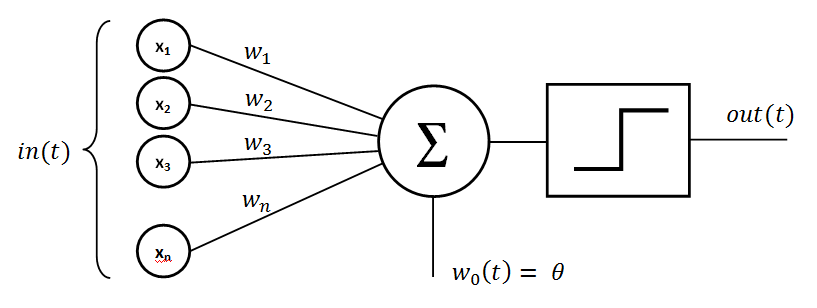
\includegraphics[width=15cm]{archivos/imagenes/perceptron.png}
	\caption[Perceptrón con entradas, pesos, y una salida escalonada.]{Perceptrón con entradas, pesos, y una salida escalonada\footnotemark.}
	\label{perceptron}
\end{figure}
\footnotetext{Puedes encontrar la imagen de de wikimedia.org en  \url{https://commons.wikimedia.org/wiki/File:Perceptron_moj.png}}                  

Ha sido demostrado mediante estudios empírico-analíticos y teóricos, que con un correcto entrenamiento del perceptrón, evitando el overfitting\footnote{El overfitting surge tras entrenar una red muy compleja con los mismos datos muchas iteraciones, de esta manera la red aprende el ruido de la muestra, y no es capaz de responder bien fuera de los datos de muestra.}, y proporcionando una cantidad suficiente de datos, que un solo perceptrón es capaz de separar los datos de cualquier problema que sea linealmente separable. Pudiendo entonces, mediante la sencilla implementación de un perceptrón, predecir patrones en cualquier campo con las condiciones mencionadas.

\section{Redes neuronales}
\label{Redes Neuronales}
Como ya hemos mencionado anteriormente, el \gls{mlp} no es capaz de resolver todo tipo de problemas. Gráficamente es fácil de entender que si el dataset del problema no es separable por rectas, el \gls{mlp} no resolverá el problema. Analíticamente se explica de la siguiente manera: cada perceptrón se entiende como un polinomio, es un sumatorio de cada peso multiplicado por cada entrada, y la suma de polinomios se puede simplificar fácilmente como un solo polinomio. Por eso es que descubrieron que usando una función de activación, esto se solucionaba, ya que gráficamente la función ya no será una recta, y analíticamente no se podrá simplificar a un solo polinomio.
Existen muchas funciones de activación, entre ellas cabe mencionar a las más usadas: la sigmoide \ref{Funcion sigmoide}, la tangente hiperbólica \ref{Funcion tangente hiperbolica}, y la ReLU \ref{Funcion ReLU}

\begin{equation}
	\label{Funcion sigmoide}
	f(x) =  \frac{\mathrm{1} }{\mathrm{1} + e^{-x} }
\end{equation}
\begin{equation}
	\label{Funcion tangente hiperbolica}
	f(x) =  \frac{\mathrm{2} }{\mathrm{1} + e^{-2x} }  - 1
\end{equation}
\begin{equation}
	\label{Funcion ReLU}
	f(x)= \left\{ \begin{array}{lcc}
		0 &   si  & x < 0 \\
		\\ x &  si  & x \geq 0
	\end{array}
	\right.
\end{equation}

Esta es la principal diferencia entre una red neuronal y una \gls{mlp}, y una diferencia que hace que la \gls{ia} se haya podido extender más aún para la resolución de problemas. Algunos de estos no tienen una resolución viable debido a que la complejidad computacional del algoritmo es extremadamente alta, otros porque ni siquiera se conoce o no se puede desarrollar un algoritmo que resuelva el problema. 
\\
Pero después de entender esta maravillosa forma de resolver casi cualquier problema surge otra cuestión, ¿cómo ajustamos los pesos de la red? Si una persona tiene que encargarse de hacerlo por fuerza bruta, sería capaz para problemas pequeños, pero cuantos más parámetros libres tenga la red, más inviable será el entrenamiento de este, ya que el tiempo que empleará entrenando crecerá exponencialmente.
\\
Por esto es que se comenzó a pensar en formas de entrenamiento alternativas, por ejemplo las redes generativas \gls{gan}, que trata de dos redes, una la cuál vamos a entrenar para resolver el problema, y otra la cuál se va a encargar de evaluar si el trabajo ha sido bien hecho. Pero la forma de entrenamiento que desarrollaré en este \gls{tfg} es el \textit{backpropagation}.

\subsection{\textit{Backpropagation}}
\label{marco teorico backpropagation}
Como su nombre indica, trata de propagar el error cometido en una muestra desde el final hasta el principio, es decir, hacia atrás. En el entrenamiento supervisado, conocemos el resultado que debería obtener la red, por lo tanto si probamos con una entrada, sabremos cuánto error ha cometido, y según cuánta culpa de ese error haya tenido una de las neuronas, se corregirá sus pesos de entrada más o menos.
El \textit{backpropagation} es un gran hito en la historia de la \gls{ia} ya que, anterior a esto sólo existía la corrección por fuerza bruta, es decir, medir cuánta culpa tenía una neurona del fallo implicaba mirar qué error habían cometido las neuronas posteriores a ella. Por lo que continuaba siendo un problema de complejidad computacional exponencial inviable, sobretodo teniendo en cuenta que los recursos eran más limitados.
¿De qué trata este algoritmo que simplifica tanto el aprendizaje? El algoritmo se apoya en el descenso del gradiente que es otro algoritmo que se basa en que, para encontrar un mínimo relativo en una función haremos la derivada de esta, la derivada nos aporta la pendiente en el punto, y si le restamos la pendiente a nuestra función nos iremos aproximando cada vez más a un mínimo relativo. Pero seguimos teniendo el problema de tener que hacer los cálculos para esa neurona, y las siguientes en la red.
\\
Los ingenieros se dieron cuenta de que en la corrección durante el entrenamiento había un factor que se repetía, a este lo llamaron como la letra griega delta ($\delta$), ya que en matemáticas esta letra representa el diferencia o cambio. Por lo que para aplicar la corrección a la neurona sólo tendrías que acumular los delta de las neuronas posteriores. 

El mayor problema de este es entender cómo funciona teóricamente este, ya que en código no es muy complicado de hacer una vez entiendes los índices que componen el algoritmo. Para saber cómo se implementa el, he desarrollado un esquema que puedes ver en la figura \ref{Algoritmo de backpropagation}.
\begin{figure}[h]
	\centering
	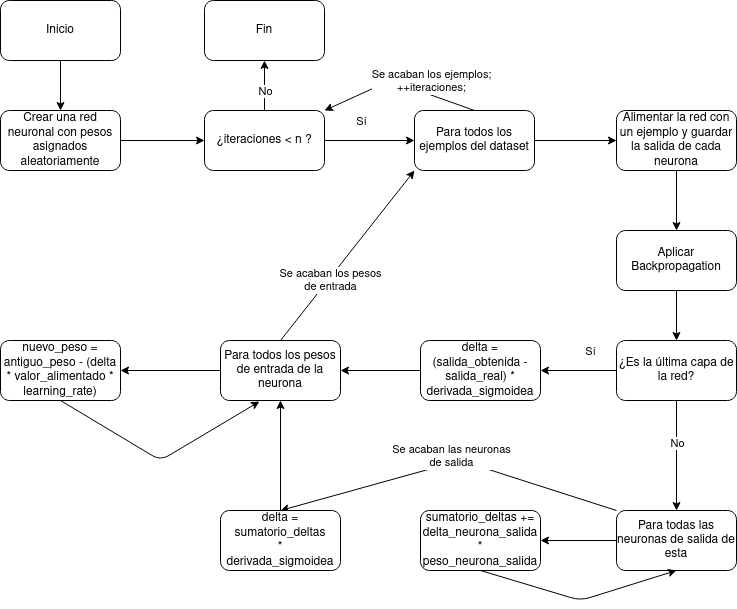
\includegraphics[width=15cm]{archivos/imagenes/Algoritmo-de-backpropagation.png}
	\caption{Algoritmo de \textit{backpropagation}.}
	\label{Algoritmo de backpropagation}
\end{figure}

Y aunque parece fácil de entender viéndolo de una forma esquemática, el problema está cuando has de saber a qué índice corresponde cada fórmula en el código. Lo que haremos será escoger un ejemplo del dataset. Para cada peso de entrada (j), de cada neurona (i), de cada capa (l), vamos a aplicar la fórmula \ref{eq:descenso del gradiente} Es decir, aplica el descenso del gradiente.
\begin{subequations}
	\begin{eqnarray}
		w_{ij}^{(l)} = w_{ij}^{(l)} - \alpha*\nabla E(w_{ij}^{(l)}) \label{eq:descenso del gradiente} \\
		\nabla E(w_{ij}^{(l)}) =  \frac{\delta E(w_{ij}^{(l)})}{\delta w_{ij}^{(l)}} \label{eq:derivada parcial}
	\end{eqnarray}
\end{subequations}
El alpha que aparece, que todavía no he comentado, es el factor de aprendizaje, que hará que el descenso del gradiente sea más rápido pero más errático si es más grande, y más lento pero preciso si es más pequeño. Y la fórmula \ref{eq:derivada parcial} representa el gradiente de la función de error, es decir, en este caso la derivada parcial respecto al peso j de la neurona i.

La función de error que estoy usando en \textit{backpropagation} es el error cuadrático, es decir, la media de la suma de los cuadrados en la fórmula \ref{Error cuadratico}. Siendo $h(x)_n$ el resultado de la red neuronal para una entrada x, $y_n$ el resultado real que debería haber obtenido, y N el número total de ejemplos. Cabe destacar que el superíndice es una ele mayúscula debido a que esto connota que la capa de la que hablamos es la última.
\begin{equation}
	\label{Error cuadratico}
	E(w_{ij}^{(L)}) = \frac{1}{N}\sum_{n=0}^N(h(x)_n - y_n)^2
\end{equation}

Pero ahora queremos calcular el gradiente del error, y para eso necesitamos saber qué es lo que vale la función \ref{eq:derivada parcial}. Para eso usaremos la regla de la cadena. Pero antes de ponernos con la fórmula, hay que entender qué significa cada símbolo. 

\begin{figure}[H]
	\centering
	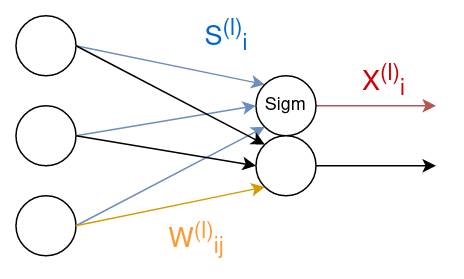
\includegraphics[width=15cm]{archivos/imagenes/Red-neuronal-simbolos.png}
	\caption{Símbolos de una red neuronal.}
	\label{fig:symb neural net}
\end{figure}

Como se puede apreciar en la figura \ref{fig:symb neural net}, la W con sus índices se refiere al peso j de una neurona i de la capa l. La S  con sus índices se refiere a la señal (sumatorio de cada entrada por cada peso) de la neurona i en la capa l. Sigm se refiere a la función de activación, la sigmoidea en este caso. Y por último x con sus índices se refiere a la salida de la neurona i (la ele minúscula indica la capa, si quisiéramos la salida de la capa anterior, que es lo que nos interesa, usaremos l-1) después de pasar por la función de activación, si fuese la capa l sería la salida de la neurona anterior.
\\
Una vez entendido cada símbolo, podemos entender la regla de la cadena que aplicamos en la fórmula \ref{Chain rule signal}. Gracias a esta regla obtenemos algo más sencillo de calcular, que es la derivada de la señal respecto al peso, mucho más sencillo de calcular como vemos en la fórmula \ref{Derivada de la señal respecto al peso}. Y a la derivada del error respecto a la señal, es a lo que llamaremos delta, que como expliqué en el marco teórico, es lo que se acumula en todas las capas, y por lo tanto lo que nos va a interesar almacenar.
\begin{subequations}
	\begin{eqnarray}
		\nabla E(w_{ij}^{(l)}) =  \frac{\delta E(w_{ij}^{(l)})}{\delta w_{ij}^{(l)}} = \frac{\delta E(w_{ij}^{(l)})}{\delta w_{ij}^{(l)}} * \frac{\delta S_{i}^{(l)}}{\delta S_{i}^{(l)}} = \frac{\delta E(w_{ij}^{(l)})}{\delta S_{i}^{(l)}} * \frac{\delta S_{i}^{(l)}}{\delta w_{ij}^{(l)}} \label{Chain rule signal} \\
		\frac{\delta S_{i}^{(l)}}{\delta w_{ij}^{(l)}} = \frac{\delta (x_{i}^{(l-1)}*w_{ij}^{(l)}) }{\delta w_{ij}^{(l)}} = x_{i}^{(l-1)} \label{Derivada de la señal respecto al peso}
	\end{eqnarray}
\end{subequations}

Pero todavía no sabemos lo que vale delta, así que volvemos a aplicar la regla de la cadena \ref{Chain rule delta}. Lo que conseguimos es obtener la derivada de la salida de la neurona después de aplicar la función de activación, respecto al sumatorio de cada entrada de la neurona por cada peso, esto es lo mismo que la derivada de la función de activación en la señal \ref{Derivada de la salida respecto a la entrada}. Y ahora ya sí que podemos obtener la derivada de la función de error respecto a la salida de la neurona \ref{Derivada de la salida de la red respecto a la salida real}.
\begin{subequations}
	\begin{eqnarray}
		\frac{\delta E(w_{ij}^{(l)})}{\delta S_{i}^{(l)}} = \frac{\delta E(w_{ij}^{(l)})}{\delta S_{i}^{(l)}} * \frac{\delta x_{i}^{(l)}}{\delta x_{i}^{(l)}} = \frac{\delta E(w_{ij}^{(l)})}{\delta x_{i}^{(l)}} * \frac{\delta x_{i}^{(l)}}{\delta S_{i}^{(l)}} \label{Chain rule delta} \\
		\frac{\delta x_{i}^{(l)}}{\delta S_{i}^{(l)}} = Sigm'(S_{i}^{(l)}) = Sigm(S_{i}^{(l)}) * (1 - Sigm(S_{i}^{(l)})) \label{Derivada de la salida respecto a la entrada} \\
		\frac{\delta E(w_{ij}^{(l)})}{\delta x_{i}^{(l)}} = \frac{\delta (h(x) - y)^2}{\delta x_{i}^{(l)}} = \frac{\delta (x_{i}^{(l)} - y_{i})^2}{\delta x_{i}^{(l)}} = 2 * (x_{i}^{(l)} - y_{i}) \label{Derivada de la salida de la red respecto a la salida real}
	\end{eqnarray}
\end{subequations}

Por lo tanto podemos concluir que el cálculo de delta, cuando estamos en la última capa L (ele mayúscula), es la fórmula \ref{Delta en la ultima capa}. Y que el gradiente para la última capa será \ref{Gradiente para las neuronas de la ultima capa}.
\begin{subequations}
	\begin{eqnarray}
		\delta_{i}^{(L)} = 2 * (x_{i}^{(L)} - y_{i}) * Sigm(S_{i}^{(L)}) * (1 - Sigm(S_{i}^{(L)})) \label{Delta en la ultima capa} \\
		\nabla E(w_{ij}^{(l)}) = \delta_{i}^{(L)}  * x_{i}^{(L-1)} \label{Gradiente para las neuronas de la ultima capa}
	\end{eqnarray}
\end{subequations}

Pero nos faltaría calcular el gradiente para las capas anteriores a la última. Como he mencionado antes, la virtud de \textit{backpropagation} es que vamos acumulando delta porque se propaga desde el final hasta el principio. Sólo tenemos que seguir la fórmula \ref{Chain rule signal}, es decir, multiplicar el nuevo delta (que todavía no conocemos y habremos de calcular) por la entrada que corresponde a ese peso. 
\\
Por lo tanto, ya sabemos cuál es la entrada de la señal  de entrada de la neurona que corresponde a ese peso \ref{Derivada de la señal respecto al peso}, y calcular el nuevo delta, usando la regla de la cadena, y teniendo en cuenta el delta de la capa posterior, sería: la derivada de la función de activación en la señal de entrada, por el delta de la neurona de salida, por el peso que conecta esa neurona con la neurona de salida \ref{Delta en el resto de capas}. 
\\
Para entender mejor de forma visual cómo se calcula el delta de la capa l, puedes ver la figura \ref{Delta en la capa l}. Se observa como, en este caso hay dos neuronas de salida que han tenido un error, acumulado en su delta, cada delta es multiplicado por el peso que le une a esa neurona porque si el peso es mayor, significa que tendrá más culpa del error, y también se aprecia que sigue apareciendo la señal de entrada de la neurona y la derivada de la sigmoidea, porque también han afectado al error y hay que tenerlo en cuenta para el nuevo delta.
\begin{subequations}
	\begin{eqnarray}
		\delta_{i}^{(l)} = Sigm'(S_{i}^{(l)}) * \sum_{j=0}^{n} \delta_{ij}^{(l+1)} * w_{ij}^{(l+1)} \label{Delta en el resto de capas} \\
		\nabla E(w_{ij}^{(l)}) = \delta_{i}^{(l)}  * x_{i}^{(l-1)} \label{Gradiente para las neuronas del resto de capas}
	\end{eqnarray}
\end{subequations}

\begin{figure}[H]
	\centering
	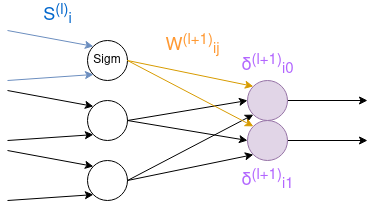
\includegraphics[width=15cm]{archivos/imagenes/Calculo-del-delta-en-la-capa-l.png}
	\caption{Cálculo de delta en la capa l $\neq$ L}
	\label{Delta en la capa l}
\end{figure}

Haremos esta operación para cada peso de cada neurona de esta capa, a ese peso le aplicaremos el gradiente como en la fórmula \ref{eq:descenso del gradiente}, y avanzaremos hacia la capa de atrás hasta que no queden más capas.

Para ver las ventajas de \textit{backpropagation} de forma empírica respecto al algoritmo aleatorio, ir al apartado de resultados (\ref{resultados}).

\subsection{Dimensión Vapnik-Chervonenkis}
Ahora sólo nos falta saber cuántos ejemplos tendremos que aportarle a la red neuronal para estar seguros de que ha aprendido. Nunca podremos asegurar que la red neuronal habrá aprendido a generalizar, ya que esto dependerá del ruido que contenga el conjunto de ejemplos. Además, aunque generalice lo que contiene el dataset, puede que no sea capaz de predecir por culpa de lo caótico que sea el sistema (como por ejemplo la bolsa de valores). Pero siempre que el sistema que tratamos de predecir sea generalizable, lo que es seguro es que cuantos más datos de ejemplo dispongamos, mejor generalizará la red. 
\\
Para esto existe una métrica llamada dimensión Vapnik-Chervonenkis, que recibe el nombre de sus dos creadores Vladimir Vapnik y Alexey Chervonenkis. Esta métrica no es exclusiva de las redes neuronales, pero es aplicable y por eso nos interesa. Explicado de forma simple quiere decir que: si una función tiene n términos independientes (el número de pesos de la red neuronal en nuestro caso), el sistema necesitará n*10 muestras de ejemplo por cada acción que quiera aprender. Es decir, si quiere aprender a pulsar arriba, abajo, o disparar (tres acciones distintas) y la red neuronal consta de 20 pesos, su dimensión Vapnik-Chervonenkis es 20, y se necesitará como mínimo 20*10*3 muestras de ejemplo para asegurar que la red ha aprendido a generalizar.

La explicación más extendida puedes encontrarla en el libro de \cite{LearningFromData}.\footnote{Más concretamente, puedes saber más sobre la dimensión Vapnik-Chervonenkis, en este vídeo del curso de Yaser Abu-Mostafa \url{https://www.youtube.com/watch?v=Dc0sr0kdBVI}}

\section{Estado del Arte}
Entre los proyectos ya hechos con anterioridad a mi \gls{tfg} existen otros \gls{tfg} de compañeros de la \gls{ua}, entre los que cabe mencionar por su similitud, son los de \cite{tfg-ia-1}, \cite{tfg-ia-2}, \cite{tfg-ia-3} y \cite{tfg-ia-4}. Los cuales se pueden encontrar en los enlaces de la bibliografía.

\subsection{Motor de videojuegos}
Pero esto no es todo. Estos trabajos anteriormente mencionados tienen algo en común, a parte de pertenecer al mundo de la \gls{ia} y los videojuegos, todos están hechos utilizando un motor de videojuegos. Y como el objetivo de este \gls{tfg} no es solo crear el videojuego y la \gls{ia} sino también aprender el funcionamiento interno de cada uno de ellos, he necesitado seguir el curso de mi tutor \cite{CursoMotorC++} , en el cual explica y crea un motor de videojuegos desde cero, tan solo usando una librería de C para abrir ventanas \footnote{TinyPTC: descargable en el siguiente enlace \url{http://bit.ly/tinyPTC-UA19}} y otra en C++ para leer los sprites que se usarán en el juego\footnote{PicoPNG: descargable en el siguiente enlace \url{http://bit.ly/picoPNG-UA19}}.
\\
Como complemento a este motor que se explica en el curso, también usaré la librería Dear ImGui\footnote{ImGUI: descargable en el siguiente enlace \url{https://github.com/ocornut/imgui}}, que es una librería de código abierto usada por grandes empresas para la renderización de ventanas, texto, botones, y demás elementos necesarios para hacer una interfaz en un juego\footnote{Algunas de las empresas son Ubisoft, Supercell, Blizzard, etc. Todas en \url{https://github.com/ocornut/imgui/wiki/Software-using-dear-imgui}}. Así que a mitad del proyecto, cuando este esté avanzado y tenga que hacer las interfaces y los menús, cambiaré TinyPTC por OpenGL para poder usar Dear ImGui en el juego.

Aunque el motor que voy a usar es de desarrollo propio, obviamente la idea no surge originalmente de mi cabeza, sino que el hecho de separar el motor del videojuego es algo que existe desde hace décadas. Por eso cabe hablar sobre algunos motores ya mencionados:

\begin{description}
	\item[Unity:] Es el motor más usado para el desarrollo de juegos indie, por varios motivos. Entre ellos son su creación hace ya muchos años, en 2005, su compatibilidad para compilar un mismo juego para una cantidad muy grande de plataformas y, posiblemente lo más importante es que, debido a su antigüedad y al ser de los primeros en ofrecerse al público de forma gratuita, tiene una comunidad enorme que permite a los desarrolladores encontrar casi cualquier duda resuelta en Internet.
	\item[Unreal Engine:]  Es más antiguo que Unity, presentado en 1998, pero al principio fue creado principalmente para hacer juegos del género shooter en primera persona y a lo largo del tiempo se ha hecho más genérico para poder crear cualquier tipo de videojuego, y además, para una gran cantidad de plataformas. 
	\item[Godot Engine:] Este es el más nuevo de los tres, 2014. Sin embargo se ha hecho conocido porque es completamente gratuito, a diferencia de los competidores que cobran unos royalties cuando tu juego es bastante vendido. Además de que la barrera de entrada es más sencilla porque usa un lenguaje de programación propio GDScript que resulta más sencillo para principiantes. Por supuesto, también permite compilar el juego para muchas plataformas.
\end{description}

Cabe destacar que estos mencionados están desarrollados todos en C++ (aunque Unity use algo de C\#), una de las razones para esto es que este lenguaje permite al programador gestionar la memoria, cosa que es esencial en un videojuego para que el usuario que lo juegue no tenga una mala experiencia jugando debido a que en los lenguajes de programación con memoria autogestionada no tienes el control sobre cuándo va a ejecutarse el recolector de basura, cosa que ralentizaría la ejecución del juego en un momento aleatorio. Esto es problemático porque un juego es un bucle en el que cada iteración se realizan varias acciones (colisiones, renderizado, eliminado o creación de entidades, etc.) y si en mitad del juego este se detuviese, arruinaría la experiencia del usuario, por eso es mejor que sea el programador y no el compilador o intérprete el que elija cuándo crear memoria (cargar mapas, texturas, sprites, etc.) y cuándo liberarla (eliminar enemigos, destruir los mapas que ya han sido usados, etc.).

He de aclarar que un motor de videojuegos no tiene la obligación de tener un entorno de desarrollo gráfico para serlo, aunque los tres mencionados sí la tengan. Cada motor es un conjunto de herramientas que facilitan el desarrollo del videojuego, y una de ellas puede ser una interfaz como es la de Godot Engine que puede ser vista en la figura \ref{Godot interfaz}. 
\begin{figure}[H]
	\centering
	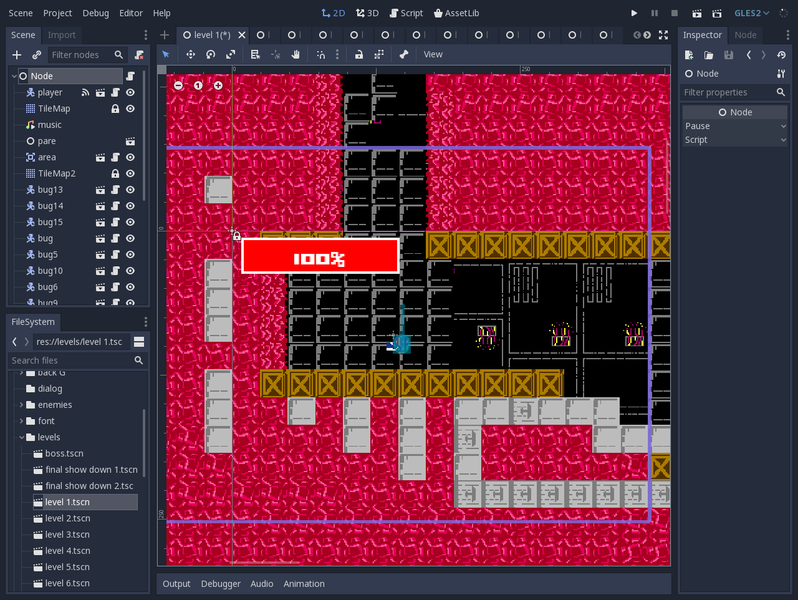
\includegraphics[width=13cm]{archivos/imagenes/Godot-captura.png}
	\caption[Interfaz de Godot.]{Interfaz de Godot\footnotemark.}
	\label{Godot interfaz}
\end{figure}
\footnotetext{Imagen extraída de Wikipedia \url{https://es.wikipedia.org/wiki/Godot}}

\subsection{\glsentrylong{ia}}
Además de los \gls{tfg} he decidido\footnote{Guiado por mi tutor, que tiene los conocimientos y experiencia en el tema necesarios para aconsejarme los documentos en los que he de fijarme.} realizar la lectura del libro \textit{Learning from Data: A Short Course} de \citefullauthor{LearningFromData}, un experto en el mundo de la Inteligencia Artificial. Un libro en el que da la iniciación, de forma teórica, al mundo del \gls{ml}, explicando el algoritmo más básico que es el perceptrón, con las fórmulas matemáticas y las propiedades estadísticas necesarias para entenderlo. Y las clases de la asignatura de Razonamiento Automático impartidas por mi tutor Francisco J. Gallego-Durán.

El \gls{ml} en videojuegos se puede usar para entrenar a un oponente del jugador, en cuyo caso es interesante definir varios niveles de dificultad. Puesto que entrenar a una máquina para que sea mejor que un humano en un juego es una tarea relativamente sencilla, la verdadera dificultad reside en que la máquina aprenda a jugar varios niveles, con los que se pueda ajustar al nivel de habilidad del jugador, de manera que siempre suponga un reto para el jugador batir a la máquina, pero que no sea tan extremadamente difícil que el jugador pierda las ganas de continuar jugando porque ha perdido el interés.
\\
Una segunda manera de usar el \gls{ml} es entrenando un agente para que bata los récords en un juego ya existente, es decir, que sustituya la posición del humano en el juego, de manera que consiga imitar o mejorar el comportamiento de un humano en el juego. Siendo el objetivo a batir un enemigo del juego, completar un mapa, o enfrentarse contra un humano. Esta segunda, es la manera que más se ha popularizado últimamente porque es algo más vistoso, y los ejemplos más conocidos son:

\begin{description}
	\item[MuZero:] Está desarrollada por DeepMind, empresa filial de  Google. Es capaz de ganar a cualquier humano jugando al Ajedrez, al Shogi y al Go.
	\item[AlphaStar:] También desarrollada por DeepMind. Es capaz de ganar a cualquier humano jugando al Star Craft, un juego de PC que trata de reunir recursos estratégicamente para combatir a tus enemigos. Se puede ver un ejemplo en la figura \ref{alphastar}.
	\item[Dino T-Rex:] Este no es una \gls{ia}, sino más bien un juego que se activa en Chrome cuando no tienes acceso a Internet. He decidido añadirlo en esta lista ya que al ser un juego tan conocido y sencillo, existen muchas personas que han decidido empezar programando su primera \gls{ia} con este, por ello, podemos encontrar muchos ejemplos simples de como entrenar a un agente en Internet. Se puede ver en la figura \ref{dino t-rex}.
	\item[Emergent Tool Use from Multi-Agent Interaction:] No se trata de ningún juego para humanos, pero es una herramienta desarrollada por OpenAI, una organización sin ánimo de lucro centrada en el desarrollo de \gls{ia} de código abierto. Trata de unos agentes que tienen que aprender a jugar al escondite, jugando dos contra dos, teniendo que aprender tanto los que pillan como los que son pillados a ganar. Estos agentes llegaron a desarrollar finalmente técnicas que explotan los fallos de las físicas del juego.\footnote{Para más información sobre el tema en el siguiente enlace se encuentra el paper \url{https://openai.com/blog/emergent-tool-use/}}
\end{description}
\begin{figure}[H]
	\centering
	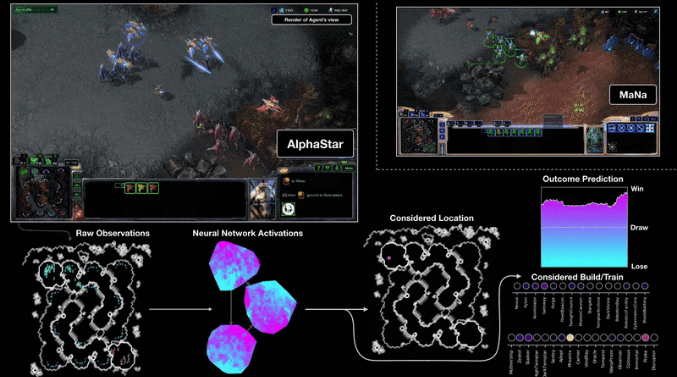
\includegraphics[width=14cm]{archivos/imagenes/alphastar-playing.png}
	\caption[Alphastar jugando al Star Craft.]{Alphastar jugando al Star Craft\footnotemark.}
	\label{alphastar}
\end{figure}
\footnotetext{En la web robologs.net \url{https://robologs.net/2019/02/03/alphastar-la-ia-de-google-aprende-a-jugar-a-starcraft-ii/}}
\begin{figure}[H]
	\centering
	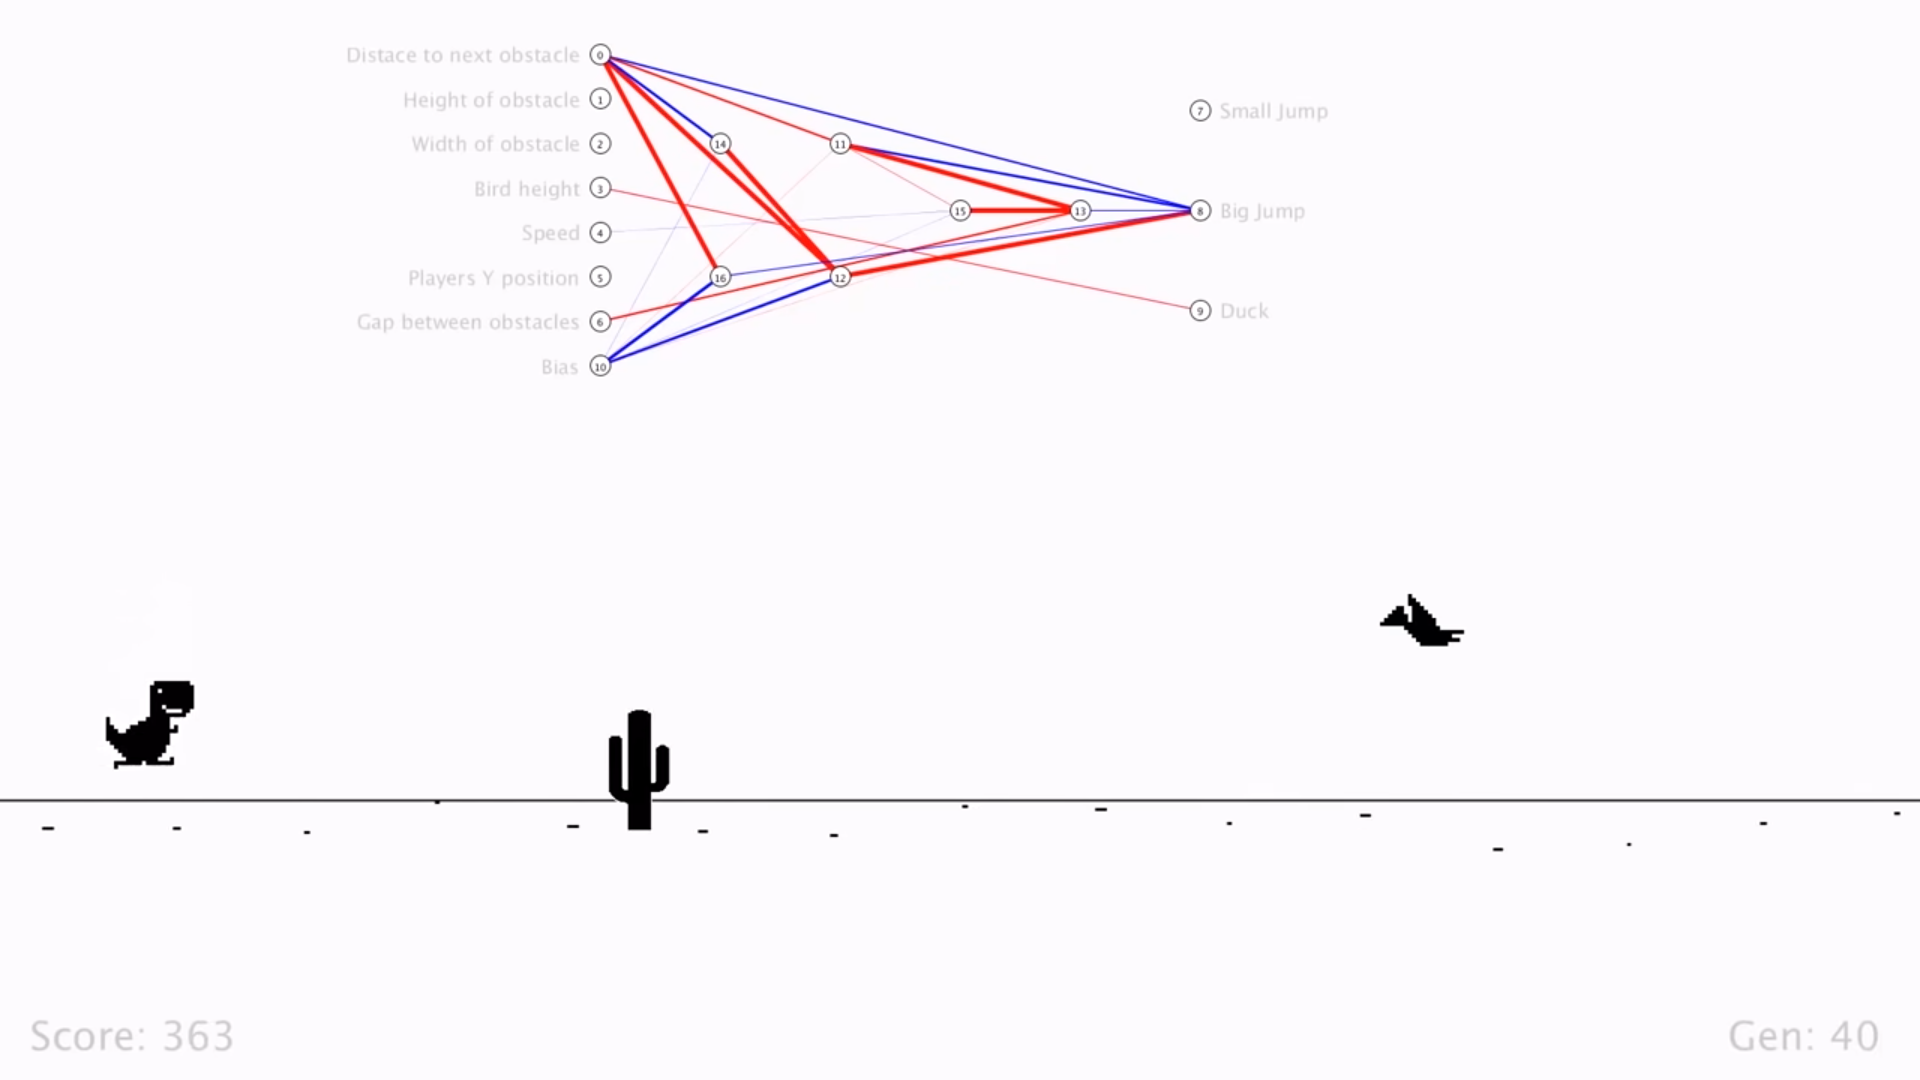
\includegraphics[width=14cm]{archivos/imagenes/dino-trex-ia.png}
	\caption[\gls{ia} aprendiendo a jugar a Dino T-Rex.]{\gls{ia} aprendiendo a jugar a Dino T-Rex\footnotemark.}
	\label{dino t-rex}
\end{figure}
\footnotetext{Del canal de YouTube de Evan Even \url{https://www.youtube.com/watch?v=sB_IGstiWlc}}